\begin{frame}
\begin{block}{equivalence of categories}
An {\it equivalence of categories}
$F : \mathcal{A} \to \mathcal{B}$ is a functor such that there
exists a functor $G : \mathcal{B} \to \mathcal{A}$ such that
the compositions $F \circ G$ and $G \circ F$ are isomorphic to the
identity functors $\text{id}_\mathcal{B}$,
respectively $\text{id}_\mathcal{A}$.
In this case we say that $G$ is a {\it quasi-inverse} to $F$.
\end{block}
\begin{block}{}
\begin{center}
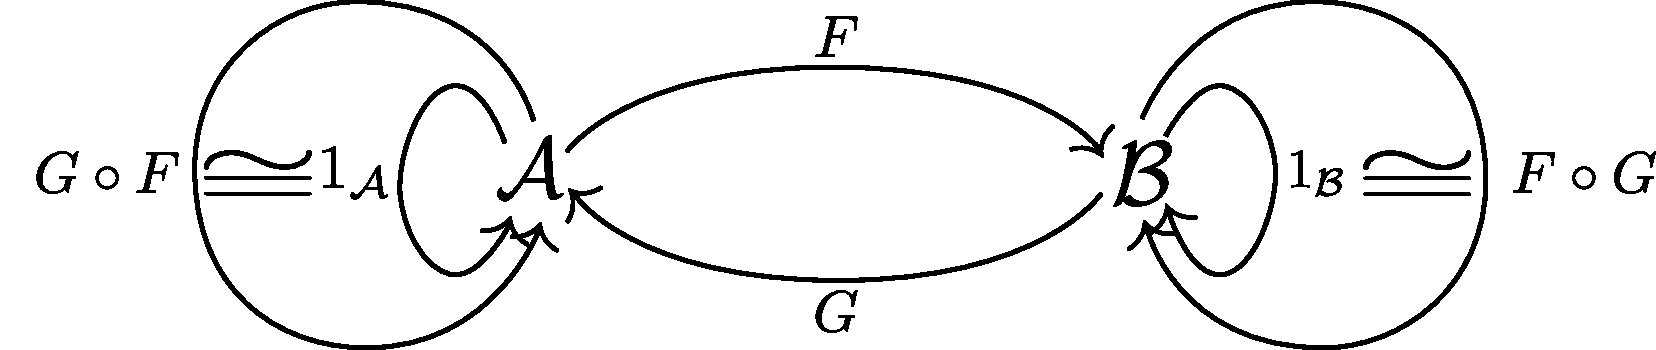
\includegraphics[width=0.6\textwidth]{fig/eqcat.pdf}
\end{center}
\end{block}
\end{frame}